% !TEX encoding = UTF-8
% !TEX TS-program = pdflatex
% !TEX root = ../tesi.tex

%**************************************************************
\chapter{Descrizione dello stage}
\label{cap:descrizione-stage}
%**************************************************************

\intro{In questo capitolo descriverò in maniera approfondita lo scopo dello stage, focalizzandomi sugli obiettivi da raggiungere e le metodologie per farlo.\\Seguirà poi una descrizione dettagliata dei casi d'uso di interesse.}\\

%**************************************************************

\section{Dominio applicativo}
\subsection{Tipi di utenti}
JGalileo CRM è stato pensato per essere utilizzato da svariate tipologie di utenti, ma a causa della grande varietà di utenti differenti che condividono però gran parte delle funzioni, i casi d'uso seguiranno solamente i due utenti più importanti:
\begin{itemize}
	\item \textbf{amministratore}: che ha il potere di creare nuovi utenti e configurare l'interfaccia finale aggiungendo e togliendo \gls{portlet}. Inoltre può accedere al pannello di controllo e monitorare la lista di utenti, modificarne i permessi e visualizzare svariate statistiche di utilizzo del prodotto;
	\item{utente semplice}, cui è permesso solamente utilizzare il software, senza aggiungere o togliere \gls{portlet} e naturalmente senza avere la possibilità di creare altri utenti.\\
\end{itemize}
	Quest'ultima è la tipologia di utenti più comune, infatti la clientela di JGalileo CRM è composta prettamente da utenti semplici, mentre solamente i membri del team di sviluppo possiedono i permessi di amministratore.
\subsection{Funzionalità}
Le funzionalità prese in esame si sviluppano soprattutto sull'interazione tra l'utente semplice e la form la cui creazione era l'obiettivo del mio stage.
Quindi i casi d'uso riguarderanno principalmente:
\begin{itemize}
	\item \textbf{inserimento di un nuova categoria di clienti};
	\item \textbf{inserimento di attività ed opportunità};
	\item \textbf{visualizzazione dettagliata dei clienti già inseriti};
	\item \textbf{visualizzazione dettagliata delle attività ed opportunità già inserite};
	\item \textbf{modifica e salvataggio dei dati};
	\item \textbf{invio di email, fax e newsletter}.
\end{itemize}
In particolare, le categorie di clienti inseribili tramite form sono:
\begin{itemize}
	\item \textbf{Leads}: Sono persone ed aziende che possono avere interesse ai prodotti e servizi dell'utente. Anche un primo contatto, come ad esempio un biglietto da visita, è considerato un lead;
	\item \textbf{Accounts}: Contengono i dati di un'azienda con cui è già presente un qualche tipo di relazione commerciale, anche solo una risposta d'acquisto;
	\item \textbf{Contatti}: I contatti consistono in persone fisiche con cui è già presente un qualche tipo di relazione commerciale. Spesso account e contatto sono in relazione tra di loro, ma è anche possibile che un contatto non abbia nessun account associato (ad esempio un privato).
\end{itemize}
mentre per attività ed opportunità si intende:
\begin{itemize}
	\item \textbf{attività}: un attività riguarda qualsiasi tipo di operazione ed evento con lo scopo di ottenere un ritorno in termini di visibilità ai clienti ed alle aziende partner.\\
	Tra le attività si inseriscono fiere, esposizioni, eventi, cene,...;
	\item \textbf{opportunità}: Le opportunità costituiscono, per il cliente che acquista JGalileo CRM, di tenere traccia delle possibilità di concludere accordi commerciali con i clienti.
\end{itemize}
Per quanto riguarda la parte di amministrazione, verrà illustrata solamente la procedura di inserimento di un nuovo utente, mentre per quanto riguarda la parte dedicata agli utenti semplici, vengono illustrate un ampio spettro di funzionalità.

%**************************************************************
\section{Casi d'uso}
I casi d'uso (use case) sono una tecnica dell'ingegneria del software per ottenere un'analisi precisa e senza ambiguità dei requisiti di un sistema, con l'obiettivo di perseguire la creazione di software di qualità.\hyperlink{23}{[23]}\\
I casi d'uso sono solitamente rappresentati in forma testuale, attraverso la descrizione dettagliata del caso d'uso stesso in termini di attori coinvolti, pre e post condizioni, e da una rappresentazione grafica, definita Use Case Diagram, con l'ausislio di un altro linguaggio, \gls{uml}\glsfirstoccur\hyperlink{03}{[03]}.\\
Tutti i casi d'uso saranno qui presentati attraverso descrizione testuale, mentre la rappresentazione grafica verrà utilizzata solamente per gli scenari più generali.\\
I casi d'uso qui riportati non si riferiscono all'intero software a causa della sua grande complessità ed ampiezza d'utilizzo, ma solamente agli scenari principali che, direttamente od indirettamente, sono influenzati dal codice da me scritto durante l'esperienza di stage.\\

\newpage

\subsection{Classificazione dei casi d'uso}
Ogni caso d’uso è classificato secondo la seguente convenzione:
\begin{center}
	UC[codice]
\end{center}
Dove [codice] è un codice numerico che identifica univocamente il caso d’uso.\\
Esso è sequenziale e gerarchico, dunque se ad esempio il caso d’uso "X" necessita di un ulteriore livello di dettaglio si procede individuando i sotto-casi d’uso "X.Y", dove:\\
\begin{itemize}
	\item \textbf{X}: il codice identificativo del caso d'uso padre, solitamente generico e difficilmente descrivibile nel dettaglio; 
	\item \textbf{Y}: codice figlio, identifica un caso d'uso più particolare rispetto al padre (che lo contiene).
	
\end{itemize}
X parte con indice 1 e valore crescente, mentre Y e Z parto dall'indice 0 con valore crescente.\\
Indicherò con il suffisso “\_G” tutti quei casi d’uso di alto livello, a segnalare che si tratta di una visione generale del contesto.
\subsection{Struttura dei casi d'uso}
Ogni caso d'uso verrà descritto in maniera testuale, utilizzando la seguente struttura:
\begin{itemize}
	\item \textbf{Attori}: Gli attori comprendono le entità umane che interagiscono con il sistema. \\ 
	Nella fattispecie, vengono distinti tre tipologie di attori:
	\begin{itemize}
		\item \textbf{Amministratore}: Questa tipologia di attore è quella riservata solamente agli sviluppatori del prodotto;
		\item \textbf{Utente non autenticato}: indica un attore non ancora autenticato nel sistema;
		\item \textbf{Utente autenticato}, indicato anche semplicemente come \textbf{Utente}, indica un utente non amministratore che viene riconosciuto dal sistema e può quindi usufruirne.
	\end{itemize}
	\item \textbf{Pre-condizione}: Indica le condizioni che devono necessariamente essere soddisfatte affinchè sia possibile l'interazione dell'attore con lo specifico caso d'uso;
	\item \textbf{Post-condizione}: Indica le condizioni in cui l'attore si verrà a trovare dopo la fine dell'interazione con lo specifico caso d'uso;
	\item \textbf{Descrizione}: Riporta una breve descrizione testuale del caso d'uso.
\end{itemize}

\newpage

\section{UC 1\_G: Funzionalità amministratore}
\begin{figure}[h]
	\centering
	\includegraphics[height = 8 cm]{/usecase/funzionalità-amm}
	\caption{Caso d'uso generale-funzionalità amministratore}
\end{figure}

\subsection{UC 1 - inserimento nuovo utente}

\begin{itemize}
	\item \textbf{Descrizione}: l'amministratore può aggiungere un nuovo utente inserendo i seguenti campi nell'apposita form:
	\begin{itemize}
		\item nome;
		\item cognome;
		\item titolo;
		\item data di nascita;
		\item sesso;
		\item occupazione.
	\end{itemize}
	\item \textbf{Attore}: Utente amministratore;
	\item \textbf{Pre-condizione}: L'amministratore ha già effettuato l'accesso tramite inserimento di username e password, ed ha raggiunto il pannello di amministrazione;
	\item \textbf{Post-condizione}: è stato inserito un nuovo utente.
\end{itemize}

\newpage

\section{UC 2\_G: Funzionalità utente - inserimento}

I casi d'uso qui riportati si riferiscono all'inserimento di nuovi dati nel sistema

\begin{figure}[h]
	\centering
	\includegraphics[height = 12 cm]{/usecase/funzionalità-utente}
	\caption{Caso d'uso generale-funzionalità utente}
\end{figure}

Negli UC 3, 4, 5, 6, 7 non vengono riportati tutti i campi inseribili, in quanto, per ogni singola form, si hanno almeno 40 differenti campi.\\

\subsection{UC 2 - Autenticazione}

\begin{itemize}
	\item \textbf{Descrizione}: per l'autenticazione è necessario inserire nel sistema:
	\begin{itemize}
		\item \textbf{nome utente};
		\item \textbf{password}.
	\end{itemize}
	\item \textbf{Attore}: Utente non autenticato;
	\item \textbf{Pre-condizione}: Un utente amministratore deve aver aggiunto l'utente che sta per effettuare l'accesso affinché l'autenticazione vada a buon fine;
	\item \textbf{Post-condizione}:l'utente viene autenticato e può utilizzarne le funzionalità del prodotto in base ai suoi permessi.
\end{itemize}

\subsection{UC 3 - Aggiunta lead}

\begin{itemize}
	\item \textbf{Descrizione}: un utente può aggiungere un lead al suo insieme di potenziali clienti. Per farlo deve inserire alcune informazioni obbligatorie, come:
	\begin{itemize}
		\item \textbf{cognome};
		\item \textbf{nome della società}.
	\end{itemize}
	e molte altre facoltative, ma che sono molto importanti al fine di avere una rapida e completa panoramica del potenziale cliente. Tra queste ci sono:
	\begin{itemize}
		\item \textbf{email};
		\item \textbf{indirizzo dell'ufficio};
		\item \textbf{descrizione del lead};
		\item \textbf{numero di cellulare};
		\item \textbf{provenienza del lead}.
	\end{itemize}
	\item \textbf{Attore}: Utente autenticato;
	\item \textbf{Pre-condizione}: Un utente deve aver eseguito l'accesso ed essersi portato alla pagina di inserimento lead;
	\item \textbf{Post-condizione}:il nuovo lead contenente le informazioni inserite viene salvato [UC 12] nel sistema ed è disponibile all'utente.
\end{itemize}

\subsection{UC 4 - Aggiunta account}

\begin{itemize}
	\item \textbf{Descrizione}: un utente può aggiungere un account alla lista di clienti. Un account può essere di vari tipi, come:
	\begin{itemize}
		\item \textbf{Prospect} (UC 4.1): un prospect rappresenta una potenziale azienda cliente, con la quale non si è ancora aperto alcun tipo di rapporto commerciale;
		\item \textbf{Partner} (UC 4.2):un partner consiste in un'azienda con cui si è stabilito un duraturo rapporto di scambi, eventualmente anche non solo commerciali;
		\item \textbf{Organizzazione} (UC 4.3):un organizzazione consiste in un'insieme di persone e mezz, volti ad uno stesso obiettivo comune;
		\item \textbf{Concorrente} (UC 4.4): questo tipo di account si riferisce ad un'azienda che opera nello stesso settore del cliente, in concorrenza con esso.
	\end{itemize}
   Questi tipi di account hanno form che utilizzano campi dati anche molto diversi tra loro, a causa della differente e talvolta profonda natura che li connota, ma anche taluni campi in comune, come:
   \begin{itemize}
   		\item \textbf{Ragione sociale};
		\item \textbf{indirizzo};
		\item \textbf{numero di telefono};
		\item \textbf{città};
		\item \textbf{partita IVA}.
	\end{itemize}
	\item \textbf{Attore}: Utente autenticato;
	\item \textbf{Pre-condizione}: Un utente deve aver eseguito l'accesso ed essersi portato alla pagina di inserimento account;
	\item \textbf{Post-condizione}:il nuovo account contenente le informazioni inserite viene salvato nel sistema [UC 12] ed è disponibile all'utente.
\end{itemize}

\subsection{UC 5 - Aggiunta contatto}

\begin{itemize}
	\item \textbf{Descrizione}: un utente può aggiungere un contatto al sistema. Per farlo deve inserire alcune informazioni obbligatorie, come:
	\begin{itemize}
		\item \textbf{cognome};
		\item \textbf{account da associare al contatto}.
	\end{itemize}
	e molte altre facoltative, tra le quali:
	\begin{itemize}
		\item \textbf{email};
		\item \textbf{indirizzo dell'ufficio};
		\item \textbf{qualifica del contatto};
		\item \textbf{stabilimento di lavoro del contatto}.
	\end{itemize}
	\item \textbf{Attore}: Utente autenticato;
	\item \textbf{Pre-condizione}: Un utente deve aver eseguito l'accesso ed essersi portato alla pagina di inserimento contatto;
	\item \textbf{Post-condizione}:il nuovo contatto contenente le informazioni inserite viene salvato nel sistema [UC 12] ed è disponibile all'utente.
\end{itemize}

\subsection{UC 6 - Aggiunta attività}

\begin{itemize}
	\item \textbf{Descrizione}: un utente può aggiungere un'attività alla lista di attività già inserite in precedenza. Per farlo deve inserire alcune informazioni obbligatorie, come:
	\begin{itemize}
		\item \textbf{descrizione}: una piccola descrizione testuale dell'attività;
	\end{itemize}
	e molte altre facoltative, tra le quali:
	\begin{itemize}
		\item \textbf{sede della visita};
		\item \textbf{account e contatti associati};
		\item \textbf{data d'inizio};
		\item \textbf{data di fine}.
	\end{itemize}
	\item \textbf{Attore}: Utente autenticato;
	\item \textbf{Pre-condizione}: Un utente deve aver eseguito l'accesso ed essersi portato alla pagina di inserimento attività;
	\item \textbf{Post-condizione}:la nuova attività contenente le informazioni inserite viene salvata nel sistema [UC 12] ed è disponibile all'utente.
\end{itemize}

\subsection{UC 7 - Aggiunta opportunità} %TODO


\begin{itemize}
	\item \textbf{Descrizione}: un utente può aggiungere un'opportunità alla lista di opportunità create in precedenza. Per farlo deve inserire alcune informazioni obbligatorie, come:
	\begin{itemize}
		\item \textbf{nome utente};
		\item \textbf{password}.
	\end{itemize}
	e molte altre facoltative, tra le quali:
	s\begin{itemize}
		\item \textbf{nome utente};
		\item \textbf{password}.
	\end{itemize}
	\item \textbf{Attore}: Utente autenticato;
	\item \textbf{Pre-condizione}: Un utente deve aver eseguito l'accesso ed essersi portato alla pagina di inserimento opportunità;
	\item \textbf{Post-condizione}:la nuova opportunità contenente le informazioni inserite viene salvata nel sistema [UC 12] ed è disponibile all'utente.
\end{itemize}

\section{UC 3\_G - Visualizzazione dettagli}

Questi casi d'uso si riferiscono alla visualizzazione ed eventuale modifica di schede di leads, account, contatti ed opportunità già inserite. 

\begin{figure}[h]
	\centering
	\includegraphics[height = 9 cm]{/usecase/funzionalità-estese}
	\caption{Caso d'uso generale 3 - visualizzazione dettagli dei dati già inseriti}
\end{figure}

\subsection{UC 8 - Visualizzazione dettaglio lead}

\begin{itemize}
	\item \textbf{Descrizione}: un utente può vedere nel dettaglio le informazioni inserite a proposito di un cliente lead. Può eventualmente aggiornarne le informazioni, eliminarlo oppure mandare una mail od un fax, come evidenziato negli [UC 12], [UC 13], [UC 14], [UC 15], [UC 16] ed [UC 17].\\
	\item \textbf{Attore}: Utente autenticato;
	\item \textbf{Pre-condizione}: Un utente deve aver eseguito l'accesso, essersi portato alla pagina riguardante i lead ed averne selezionato uno;
	\item \textbf{Post-condizione}:il lead eventualmente modificato viene salvato nel sistema per una prossima interazione.
\end{itemize}

\subsubsection{UC 8.1 - Conversione lead} %TODO

\begin{itemize}
	\item \textbf{Descrizione}: un utente può convertire il lead: In fase di inserimento, infatti, un lead viene di default salvato come "non convertito".
	\item \textbf{Attore}: Utente autenticato;
	\item \textbf{Pre-condizione}: Un utente deve aver eseguito l'accesso, essersi portato alla pagina riguardante i lead, averne selezionato uno ed essere quindi entrato nella pagina del dettaglio;
	\item \textbf{Post-condizione}:il lead viene convertito e le informazioni riguardo ad esso non sono più modificabili.
\end{itemize}

\subsection{UC 9 - Visualizzazione dettaglio account}

\begin{itemize}
	\item \textbf{Descrizione}: un utente può vedere nel dettaglio le informazioni relative ad un account in particolare. Può eventualmente aggiornarne le informazioni, eliminarlo oppure mandare una mail od un fax, come evidenziato negli [UC 12], [UC 13], [UC 14], [UC 15], [UC 16] ed [UC 17].\\
	\item \textbf{Attore}: Utente autenticato;
	\item \textbf{Pre-condizione}: Un utente deve aver eseguito l'accesso, essersi portato alla pagina relativa agli account ed averne selezionato uno;
	\item \textbf{Post-condizione}:l'account eventualmente modificato viene salvato nel sistema per una prossima interazione.
\end{itemize}

\subsection{UC 10 - Visualizzazione dettaglio contatto}

\begin{itemize}
	\item \textbf{Descrizione}: un utente può vedere le informazioni relative ad un contatto precedentemente inserito nel sistema e può eventualmente modificarlo, inviare mail o fax, come evidenziato in [UC 12], [UC 13], [UC 14], [UC 15], [UC 16] ed [UC 17].\\
	\item \textbf{Attore}: Utente autenticato;
	\item \textbf{Pre-condizione}: Un utente deve aver eseguito l'accesso, essersi portato alla pagina di inserimento contatto ed averne selezionato uno;
	\item \textbf{Post-condizione}:il contatto eventualmente modificato viene salvato nel sistema per una prossima interazione.
\end{itemize}

\subsection{UC 11 - Visualizzazione dettaglio opportunità}

\begin{itemize}
	\item \textbf{Descrizione}: un utente può vedere ed eventualemnte modificare le informazioni riguardanti una specifica opportunità. Le azioni disponibili per le opportunità sono descritte nei casi  d'uso [UC 12], [UC 13], [UC 14], [UC 15], [UC 16] ed [UC 17].\\
	\item \textbf{Attore}: Utente autenticato;
	\item \textbf{Pre-condizione}: Un utente deve aver eseguito l'accesso, essersi portato nella pagina relativa alle opportunità ed averne selezionata una;
	\item \textbf{Post-condizione}:l'opportunità eventualmente aggiornata viene salvata nel sistema per una successiva interazione.
\end{itemize}

\subsubsection{UC 11.1 - Aggiunta nota} %TODO

\begin{itemize}
	\item \textbf{Descrizione}: %TODO
	\item \textbf{Attore}: 
	\item \textbf{Pre-condizione}:
	\item \textbf{Post-condizione}:
\end{itemize}

\newpage

\section{UC 4\_G - Azioni comuni}

Questo paragrafo si riferisce alle azioni che è possibile compiere sulle categorie di clienti come lead, account e contatti e sulle schede di attività ed opportunità.\\
La scelta di riportarle come caso d'uso indipendenti deriva dalla volontà di evitare ripetizioni verbose e migliorare la leggibilità dei diagrammi \gls{umlg}.\\
\begin{figure}[h]
	\centering
	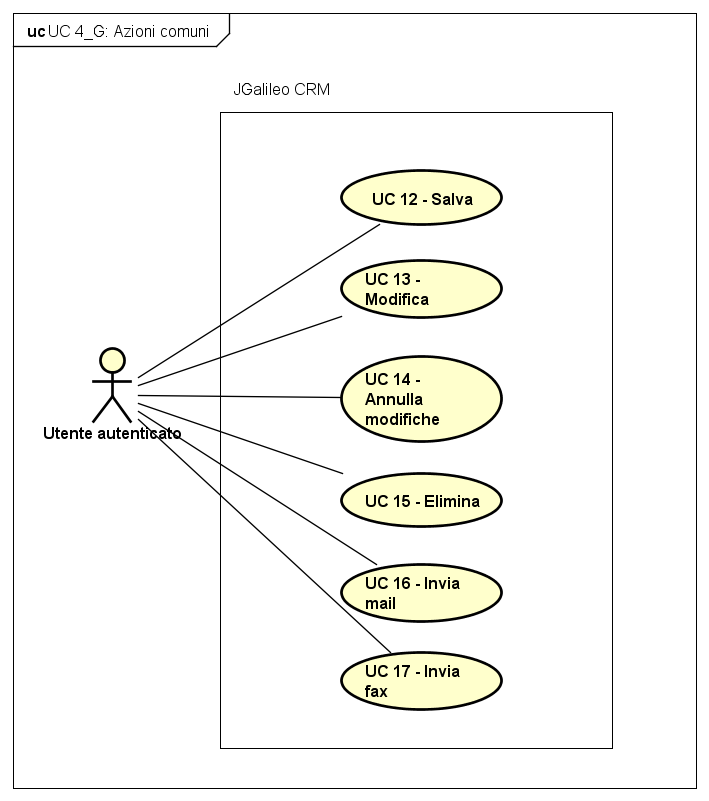
\includegraphics[height = 9 cm]{/usecase/azioni-comuni}
	\caption{Caso d'uso generale 4 - azioni comuni alle categorie sopra descritte}
\end{figure}
Per facilitare il riferimento ad un qualsiasi lead, account, contatto, attività ed opportunità precedentemente inserito nel sistema oppure in fase di inserimento verrà utilizzato il termine \textbf{scheda}.
\subsection{UC 12 - Salva}

\begin{itemize}
	\item \textbf{Descrizione}: un utente può confermare di voler inserire i dati appena immessi nel sistema o salvare le modifiche fatte ad una scheda. \\
	 in particolare i dati vengono salvati nel database AS/400.
	\item \textbf{Attore}: Utente autenticato;
	\item \textbf{Pre-condizione}: Un utente deve aver eseguito l'accesso, essersi portato ad una pagina di inserimento o di visualizzazione dettaglio ed avere inserito le informazioni obbligatorie oppure modificato almeno un campo rispetto ad una scheda preesistente;
	\item \textbf{Post-condizione}:viene notificato il corretto inserimento nel sistema oppure le corretta modifica di dati precedentemente inseriti.
\end{itemize}

\subsection{UC 13 - Modifica}

\begin{itemize}
	\item \textbf{Descrizione}: un utente può modificare le informazioni riguardanti una specifica scheda.
	\item \textbf{Attore}: Utente autenticato;
	\item \textbf{Pre-condizione}: Un utente deve aver eseguito l'accesso ed avere aperto una specifica scheda di suo interesse;
	\item \textbf{Post-condizione}:l'utente è ora abilitato alla modifica dei campi su cui è premessa la modifica.
\end{itemize}

\subsection{UC 14 - Annulla modifiche}

\begin{itemize}
	\item \textbf{Descrizione}: un utente può annullare le modifiche eventualmente apportate ad una scheda, riportandola allo stato in cui è salvata sul database;
	\item \textbf{Attore}: Utente autenticato;
	\item \textbf{Pre-condizione}: Un utente deve aver eseguito l'accesso, avere aperto una specifica scheda di suo interesse ed averne modificato almeno un campo;
	\item \textbf{Post-condizione}:la scheda viene ripulita da tutte le modifiche e ritorna quindi allo stato in cui è stata recuperata dal database.
\end{itemize}

\subsection{UC 15 - Elimina}

\begin{itemize}
	\item \textbf{Descrizione}: un utente può eliminare una scheda precedentemente inserita;
	\item \textbf{Attore}: Utente autenticato;
	\item \textbf{Pre-condizione}: Un utente deve aver eseguito l'accesso ed avere aperto una specifica scheda di suo interesse;
	\item \textbf{Post-condizione}:I dati relativi alla scheda in esame vengono eliminati dal database e non sono quindi più disponibili.
\end{itemize}

\subsection{UC 16 - Invia mail}

\begin{itemize}
	\item \textbf{Descrizione}: un utente può inviare una email all'indirizzo email presente nella scheda, se questo è stato inserito;
	\item \textbf{Attore}: Utente autenticato;
	\item \textbf{Pre-condizione}: Un utente deve aver eseguito l'accesso ed avere aperto una specifica scheda di suo interesse;
	\item \textbf{Post-condizione}:L'utente viene reindirizzato ad una pagina in cui può scrivere la mail e può, tramite una form, inserire ulteriori informazioni.
\end{itemize}

\subsection{UC 17 - Invia fax}

\begin{itemize}
	\item \textbf{Descrizione}: un utente può inviare un fax al numero di fax presente nella scheda, se questo è stato inserito;
	\item \textbf{Attore}: Utente autenticato;
	\item \textbf{Pre-condizione}: Un utente deve aver eseguito l'accesso ed avere aperto una specifica scheda di suo interesse;
	\item \textbf{Post-condizione}:L'utente viene reindirizzato ad una pagina in cui può scrivere il fax e può, tramite una form, inserire ulteriori informazioni.
\end{itemize}

\section{Tracciamento dei requisiti}
\subsection{Struttura di un requisito}
Ogni requisito identificato è stato classificato come segue:
\begin{center}
	R[Importanza][Classificazione][Identificativo]
\end{center}
\begin{itemize}
	\item \textbf{Importanza:} Specifica il grado di necessità che il requisito possiede, si articola in:
	\begin{itemize}
		\item \textbf{O (Obbligatorio)}: Il suo soddisfacimento è essenziale alla buona riuscita del progetto;
		\item \textbf{D (Desiderabile)}: Il suo soddisfacimento non è necessario ma offre funzionalità tali da renderlo uno dei primi requisiti da soddisfare in sviluppi successivi;
		\item \textbf{F (Funzionale)}: Il valore aggiunto dato dal soddisfacimento di questo requisito non è così importante, quindi prima di soddisfare il requisito è consigliata un’analisi di tempi e costi per evitare ritardi nella consegna e/o costi superiori a quelli preventivati.
	\end{itemize}
	\item \textbf{Classificazione}: Indica il tipo del requisito, in termini di finalità dello stesso:
	\begin{itemize}
		\item \textbf{F (Funzionali)}: indica una funzionalità che il prodotto deve avere; 
		\item \textbf{Q (Qualità)}: indica un requisito che riguarda l'aspetto qualitativo del prodotto;
		\item \textbf{V (Vincolo)}: indica un vincolo che deve essere rispettato durante lo sviluppo del prodotto.
	\end{itemize} 
	\item \textbf{Identificativo}: Un codice numerico crescente a partire da 1 e che identifica un requisito in modo univoco. 
\end{itemize}

\newpage

\subsection{Tracciamento dei requisiti}
Le tabelle \ref{tab:requisiti-funzionali} ,\ref{tab:requisiti-di-qualità} e \ref{tab:requisiti-di-vincolo} illustrano il codice del requisito, una breve descrizione testuale e lo stato di completamento alla fine dell'esperienza di stage. \\

\subsection*{Requisiti funzionali}
\begin{longtable}[h]{|p{2.5cm}|p{8cm}|p{2.5cm}|}
	\caption{Requisiti funzionali}\\
	\label{tab:requisiti-funzionali}\\
	\hline
	\rule[-4mm]{0mm}{1cm}	
	\textbf{Requisito} & \textbf{Descrizione} & \textbf{Stato}\\
	\hline
	\rule[-3mm]{0mm}{0.8cm}	
	ROF01&Un utente può compilare la form per l'inserimento di un nuovo lead&Completato\\
	\hline
	\rule[-3mm]{0mm}{0.8cm}
	ROF02&Un utente può salvare un nuovo lead&Completato\\
	\hline
	\rule[-3mm]{0mm}{0.8cm}
	ROF03&Il sistema, in fase di salvataggio, deve validare il nuovo lead &Completato\\
	\hline
	\rule[-3mm]{0mm}{0.8cm}
	ROF04&Un utente può compilare la form per l'inserimento di un nuovo prospect &Completato\\
	\hline
	\rule[-3mm]{0mm}{0.8cm}
	ROF05&Un utente può salvare un nuovo prospect&Completato\\
	\hline
	\rule[-3mm]{0mm}{0.8cm}
	ROF07&Il sistema, in fase di salvataggio, deve validare il nuovo prospect&Completato \\
	\hline
	\rule[-3mm]{0mm}{0.8cm}
	ROF07&Un utente può compilare la form per l'inserimento di un nuovo partner  & Completato\\
	\hline
	\rule[-3mm]{0mm}{0.8cm}
	ROF08&Un utente può salvare un nuovo partner&Completato\\
	\hline
	\rule[-3mm]{0mm}{0.8cm}
	ROF09&Il sistema, in fase di salvataggio, deve validare il nuovo partner&Completato \\
	\hline
	\rule[-3mm]{0mm}{0.8cm}
	ROF10&Un utente può compilare la form per l'inserimento di una nuova organizzazione  & Completato\\
	\hline
	\rule[-3mm]{0mm}{0.8cm}
	ROF11&Un utente può salvare un nuova organizzazione&Completato\\
	\hline
	\rule[-3mm]{0mm}{0.8cm}
	ROF12&Il sistema, in fase di salvataggio, deve validare la nuova organizzazione&Completato \\
	\hline
	\rule[-3mm]{0mm}{0.8cm}
	ROF13&Un utente può compilare la form per l'inserimento di un nuovo concorrente  & Completato\\
	\hline
	\rule[-3mm]{0mm}{0.8cm}
	ROF14&Un utente può salvare un nuovo concorrente&Completato\\
	\hline
	\rule[-3mm]{0mm}{0.8cm}
	ROF15&Il sistema, in fase di salvataggio, deve validare il nuovo concorrente&Completato \\
	\hline
	\rule[-3mm]{0mm}{0.8cm}
	ROF16&Un utente può compilare la form per l'inserimento di una nuova attività  & Completato\\
	\hline
	\rule[-3mm]{0mm}{0.8cm}
	ROF17&Un utente può salvare un nuova attività&Completato\\
	\hline
	\rule[-3mm]{0mm}{0.8cm}
	ROF18&Il sistema, in fase di salvataggio, deve validare la nuova attività&Completato \\
	\hline
	\rule[-3mm]{0mm}{0.8cm}
	ROF19&Un utente può compilare la form per l'inserimento di un nuovo contatto&Completato\\
	\hline
	\rule[-3mm]{0mm}{0.8cm}
	ROF20&Un utente può salvare un nuovo contatto&Completato\\
	\hline
	\rule[-3mm]{0mm}{0.8cm}
	ROF21&Il sistema, in fase di salvataggio, deve validare il nuovo contatto&Completato \\
	\hline
	\rule[-3mm]{0mm}{0.8cm}
	ROF22&Un utente può compilare la form per l'inserimento di una nuova attività  &Completato\\
	\hline
	\rule[-3mm]{0mm}{0.8cm}
	ROF23&Un utente può salvare una nuova attività&Completato\\
	\hline
	\rule[-3mm]{0mm}{0.8cm}
	ROF24&Il sistema, in fase di salvataggio, deve validare la nuova attività&Completato \\
	\hline
	\rule[-3mm]{0mm}{0.8cm}
	ROF25&Un utente può compilare la form per l'inserimento di una nuova opportunità  &Completato\\
	\hline
	\rule[-3mm]{0mm}{0.8cm}
	ROF26&Un utente può salvare una nuova opportunità&Completato\\
	\hline
	\rule[-3mm]{0mm}{0.8cm}
	ROF27&Il sistema, in fase di salvataggio, deve validare la nuova opportunità&Completato \\
	\hline
	\rule[-3mm]{0mm}{0.8cm}
	ROF28&Un utente può vedere nel dettaglio un lead precedentemente inserito&Completato\\
	\hline
	\rule[-3mm]{0mm}{0.8cm}
	ROF29&Un utente può modificare un lead precedentemente inserito&Completato\\
	\hline
	\rule[-3mm]{0mm}{0.8cm}
	ROF30&Un utente può annullare le modifiche apportate ad un lead precedentemente inserito&Completato\\
	\hline
	\rule[-3mm]{0mm}{0.8cm}
	ROF31&Un utente può eliminare un lead precedentemente inserito&Completato\\
	\hline
	\rule[-3mm]{0mm}{0.8cm}
	ROF32&Un utente può convertire un lead precedentemente inserito&Completato\\
	\hline
	\rule[-3mm]{0mm}{0.8cm}
	ROF33&Un utente può inviare una mail ad un lead precedentemente inserito&Completato \\
	\hline
	\rule[-3mm]{0mm}{0.8cm}
	ROF34&Un utente può inviare un fax ad un lead precedentemente inserito&Completato \\
	\hline
	\rule[-3mm]{0mm}{0.8cm}
	ROF35&Un utente può vedere nel dettaglio un prospect precedentemente inserito&Completato\\
	\hline
	\rule[-3mm]{0mm}{0.8cm}
	ROF36&Un utente può modificare un prospect precedentemente inserito&Completato\\
	\hline
	\rule[-3mm]{0mm}{0.8cm}
	ROF37&Un utente può annullare le modifiche apportate ad un prospect precedentemente inserito&Completato\\
	\hline
	\rule[-3mm]{0mm}{0.8cm}
	ROF38&Un utente può eliminare un prospect precedentemente inserito&Completato\\
	\hline
	\rule[-3mm]{0mm}{0.8cm}
	ROF39&Un utente può inviare una mail ad un prospect precedentemente inserito&Completato \\
	\hline
	\rule[-3mm]{0mm}{0.8cm}
	ROF40&Un utente può inviare un fax ad un prospect precedentemente inserito&Completato \\
	\hline
	\rule[-3mm]{0mm}{0.8cm}
	ROF41&Un utente può vedere nel dettaglio un prospect precedentemente inserito&Completato\\
	\hline
	\rule[-3mm]{0mm}{0.8cm}
	ROF42&Un utente può modificare un partner precedentemente inserito&Completato\\
	\hline
	\rule[-3mm]{0mm}{0.8cm}
	ROF43&Un utente può annullare le modifiche apportate ad un partner precedentemente inserito&Completato\\
	\hline
	\rule[-3mm]{0mm}{0.8cm}
	ROF44&Un utente può eliminare un partner precedentemente inserito&Completato\\
	\hline
	\rule[-3mm]{0mm}{0.8cm}
	ROF45&Un utente può inviare una mail ad un partner precedentemente inserito&Completato \\
	\hline
	\rule[-3mm]{0mm}{0.8cm}
	ROF46&Un utente può inviare un fax ad un partner precedentemente inserito&Completato \\
	\hline\rule[-3mm]{0mm}{0.8cm}
	ROF47&Un utente può vedere nel dettaglio un contatto precedentemente inserito&Completato\\
	\hline
	\rule[-3mm]{0mm}{0.8cm}
	ROF48&Un utente può modificare un contatto precedentemente inserito&Completato\\
	\hline
	\rule[-3mm]{0mm}{0.8cm}
	ROF49&Un utente può annullare le modifiche apportate ad un contatto precedentemente inserito&Completato\\
	\hline
	\rule[-3mm]{0mm}{0.8cm}
	ROF50&Un utente può eliminare un contatto precedentemente inserito&Completato\\
	\hline
	\rule[-3mm]{0mm}{0.8cm}
	ROF51&Un utente può inviare una mail ad un contatto precedentemente inserito&Completato \\
	\hline
	\rule[-3mm]{0mm}{0.8cm}
	ROF52&Un utente può inviare un fax ad un contatto precedentemente inserito&Completato \\
	\hline
	\rule[-3mm]{0mm}{0.8cm}
	ROF53&Un utente può vedere nel dettaglio un' opportunità precedentemente inserita&Completato\\
	\hline
	ROF54&Un utente può modificare un'opportunità precedentemente inserita&Completato\\
	\hline
	\rule[-3mm]{0mm}{0.8cm}
	ROF55&Un utente può annullare le modifiche apportate ad un' opportunità precedentemente inserita&Completato\\
	\hline
	\rule[-3mm]{0mm}{0.8cm}
	ROF56&Un utente può eliminare un' opportunità precedentemente inserita&Completato\\
	\hline
	\rule[-3mm]{0mm}{0.8cm}
	ROF57&Un utente può inviare una mail ad un' opportunità precedentemente inserita&Completato \\
	\hline
	\rule[-3mm]{0mm}{0.8cm}
	ROF58&Un utente può inviare un fax ad un' opportunità precedentemente inserita&Completato \\
	\hline
	\rule[-3mm]{0mm}{0.8cm}
	ROF59&Un utente può inviare una nota ad un'opportunità precedentemente inserita& Completato\\
	\hline
	\rule[-3mm]{0mm}{0.8cm}
	RDF1&Un utente può aggiungere un nuovo campo ad una form&Non completato\\
	\hline
	\rule[-3mm]{0mm}{0.8cm}
	RDF2&Un utente può eliminare un campo non obbligatorio da una form& Non completato \\
	\hline
\end{longtable}

\subsection*{Requisiti di qualità}
La seguente tabella riporta i requisiti di qualità che il software deve soddisfare:\\
\begin{table} [h]%todo
	\centering
	\caption{Requisiti di qualità}
	\label{tab:requisiti-di-qualità}
	\begin{tabular}[h]{|p{2.5cm}|p{8cm}|p{2.5cm}|}
		\hline
		\rule[-4mm]{0mm}{1cm}
		Requisito & Descrizione & Stato\\
		\hline
		\rule[-3mm]{0mm}{0.8cm}
		ROQ01&Il prototipo sviluppato deve avere le stesse funzionalità del precedente&Completato\\
		\hline
		\rule[-3mm]{0mm}{0.8cm}
		RDQ02&Il prototipo deve essere completo di CSS utilizzando il design Material&Non completato\\
		\hline	
	\end{tabular}
\end{table}

\subsection*{Requisiti di vincolo}
La seguente tabella riporta i requisiti di vincolo che devono essere rispettati durante lo sviluppo:
\begin{table}[h]
	\centering
	\caption{Requisiti di vincolo}
	\label{tab:requisiti-di-vincolo}
	\begin{tabular}[h]{|p{2.5cm}|p{8cm}|p{2.5cm}|}
		\hline
		\rule[-4mm]{0mm}{1cm}
		Requisito & Descrizione & Stato\\
		\hline
		\rule[-3mm]{0mm}{0.8cm}
		ROV01&Il sistema deve usare solamente solamente tecnologie open source&Completato\\
		\hline
		\rule[-3mm]{0mm}{0.8cm}
		ROD02&Il prodotto deve essere sviluppato cercando di appesantire il meno possibile il sistema già in uso &Completato\\
		\hline	
	\end{tabular}
\end{table}

\newpage

\section{Gli obiettivi}
Gli obiettivi del progetto di stage sono elencati nella tabella \ref{tab:obiettivi}
Essi sono classificati da:

\begin{itemize}
	\item un ID, che rappresenta univocamente l'obiettivo;
	\item un aggettivo di importanza dell'obiettivo;
	\item una breve descrizione testuale.
\end{itemize}

L'ID è formato da una lettera iniziale (P o F), ad indicare se il requisito da soddisfare sia di tipo \emph{Produttivo} o \emph{Formativo}, e da un numero sequenziale.\\
L'agettivo di importanza può essere: \emph{Obbligatorio}, \emph{Desiderabile} oppure \emph{Facoltativo}, in base alla necessità che ha lo lo stesso di essere soddisfatto.\\
La breve descrizione testuale descrive nel modo più concreto e riassuntivo possibile l'obiettivo.\\

\begin{table}[h]
	\centering
	\caption{Obiettivi dello stage}
	\label{tab:obiettivi}
	\begin{tabular}{|l|p{4cm}|p{8cm}|}
		\hline
		\rule[-4mm]{0mm}{1cm}
		ID & Importanza & Descrizione \\
		\hline
		\rule[-3mm]{0mm}{0.8cm}
		F1 & Obbligatorio & Acquisizione delle competenze di base sulla famiglia di software denominata CRM.\\
		\hline
		\rule[-3mm]{0mm}{0.8cm}
		F2 & Obbligatorio & Acquisizione delle competenze di base sul software di sviluppo GWT.\\
		\hline
		\rule[-3mm]{0mm}{0.8cm}
		F3 & Desiderabile & Acquisizione di competenze avanzate sul linguaggio di programmazione utilizzato per lo sviluppo del prototipo.\\
		\hline
		\rule[-3mm]{0mm}{0.8cm}
		P1 & Obbligatorio & Analisi dei requisiti tecnici ed applicativi.\\
		\hline
		\rule[-3mm]{0mm}{0.8cm}
		P2 & Obbligatorio & Analisi dell'User Interface.\\
		\hline
		\rule[-3mm]{0mm}{0.8cm}
		P3 & Obbligatorio & Analisi degli Use Case.\\
		\hline
		\rule[-3mm]{0mm}{0.8cm}
		P4 & Obbligatorio & Sviluppo di un prototipo che implementi le stesse funzionalità del componente esistente.\\
		\hline
		\rule[-3mm]{0mm}{0.8cm}
		P5 & Facoltativo & Implementazione di nuove funzionalità di interazione con l'utente sul prototipo sviluppato.\\
		\hline
	\end{tabular}
\end{table}

\newpage
\section {Analisi dei rischi}
Ho voluto analizzare una serie di rischi che sarebbero potuti incorrere durante il periodo di stage. Sono riassunti nella tabella\\ %todo

\begin{table}[h] %todo
	\centering
	\caption{Analisi preventiva dei rischi}
	\label{tab:analisi-dei-rischi}
	\begin{tabular}{|p{6cm}|p{5,5cm}|p{1,5cm}|}
		\hline
		\rule[-4mm]{0mm}{1cm}
		\textbf{Descrizione} & \textbf{Trattamento} & \textbf{Rischio}\\
		\hline
		La scelta di una libreria JavaScript che non soddisfacesse gli scopi dello stage avrebbe significato una grande perdita di tempo e il dover ripartire da capo con lo sviluppo & Analisi approfondita delle alternative disponibili e dialogo con il Tutor aziendale per trovare la soluzione più adeguata & Alto\\
		\hline
		La mancanza di documentazione dovuta all'adozione della metodologia agile potrebbe portare ad allungare i tempi di comprensione delle componenti & Collaborazione da parte del tutor e del team di sviluppo nel caso ci siano chiarimenti da fornire & Alto\\
		\hline
		Dovendo interagire con un software già funzionante e molto grande, le parti da me sviluppate potrebbero creare conflitti & Evitare di modificare metodi che possano essere utilizzati da altre componenti & Basso\\
		\hline
		
	\end{tabular}
\end{table}
\newpage
\cleardoublepage